%\documentclass[preprint,tightenlines,showpacs,showkeys,floatfix,
%nofootinbib,superscriptaddress,fleqn]{revtex4} 
\documentclass[tightenlines,floatfix,nofootinbib,superscriptaddress,fleqn]{revtex4-2} 
%\documentclass[aps,epsfig,tightlines,fleqn]{revtex4}
\usepackage{kotex}
\usepackage[HWP]{dhucs-interword}
\usepackage[dvips]{color}
\usepackage{graphicx}
\usepackage{bm}
%\usepackage{fancyhdr}
%\usepackage{dcolumn}
\usepackage{defcolor}
\usepackage{amsmath}
\usepackage{amsfonts}
\usepackage{amssymb}
\usepackage{amscd}
\usepackage{amsthm}
\usepackage[utf8]{inputenc}
%\pagestyle{fancy}
\usepackage{tikz}

\begin{document}

\title{\Large 2022년 2학기 물리학 II}
\author{김현철\footnote{Office: 5S-436D (면담시간 매주
    수요일-16:15$\sim$18:00)}} 
\email{hchkim@inha.ac.kr}
\affiliation{Hadron Theory Group, Department of Physics,
  Inha  University, Incheon 22212, Republic of Korea }
  \author{HuiJae-Lee} 
\email{hjlee6674@inha.edu}
\affiliation{Hadron Theory Group, Department of Physics,
  Inha  University, Incheon 22212, Republic of Korea }
\date{Autumn Semester, 2022}

\maketitle



\section*{\large Quiz 3}
\noindent {\bf 문제 1 [10pt].} 아래 질문에 답하세요.
\begin{itemize}
\item[(가)] 점전하가 만드는 전기장을 이용해서 가우스 법칙을 유도하세요.
\item[(나)] 도체 내부에서 전기장이 0이 됨을 설명하세요.
\item[(다)] 면전하밀도 $\sigma$로 대전되어 있고 무한히 큰 평면이 
  만드는 전기장의 크기는 $\sigma/2\varepsilon_0$입니다. 각각 양전하와
  음전하로 대전되어 있는 무한히 큰 평면 두 개가 거리 $d$ 만큼 떨어져서
  나란히 마주 보고 있을 때, 이 두 평면 사이에서 전기장을 구하세요. 
\end{itemize}
\vspace{0.5cm}

\noindent{\bf 풀이 : }
\begin{itemize}
  \item[(가)] 점전하의 전하를 $q$라 하고 이 점전하는 원점에 위치해 있다고 하자. 
  쿨롱의 법칙에 의해 이 점전하가 만드는 전기장 $\vec{E}$는
  \begin{align}
    \vec{E} = \frac{1}{4\pi\epsilon_0}\frac{q}{r^2}\hat{r}
  \end{align}
이다. 여기서 $\hat{r}$은 단위 벡터이다. 가우스 법칙을 유도하기 위해
중심이 원점이고 반지름이 $a$인 구를 통과하는 전기장의 플럭스 $\Phi_E$를 구해볼 것이다.
중심이 원점이고 반지름이 $a$인 구에 대해 면적분하여 구를 통과하는 전기장 $\vec{E}$의 
플럭스 $\Phi_E$는 정의에 의해 
\begin{align}\label{eq:1-1}
  \Phi_E=\oint \vec{E}\,d\vec{A}
\end{align}
으로 쓸 수 있다. $d\vec{A}$는 구에 대한 미소 면적으로 구면 좌표계를 도입하여 쓰면
\begin{align}
  d\vec{A} = a^2\sin\theta\,d\theta d\phi\,\hat{r}
\end{align}
이다. $\theta$는 $\hat{r}$과 $z$축이 이루는 각도이고 $\phi$는 $\hat{r}$을 $xy$평면에 정사영
내린 것과 $x$축이 이루는 각도이다. 적분범위는 구를 이루어야 하므로 $0<\theta<\pi$, 
$0<\phi<2\pi$이다. 따라서 플럭스 $\Phi_E$에 대한 식~(\ref{eq:1-1})는 다음과 같이
계산할 수 있다.
\begin{align}
  \begin{split}
    \Phi_E&=\int^{2\pi}_0\int^{\pi}_0 \frac{1}{4\pi\epsilon_0}\frac{q}{a^2}
    a^2\sin{\theta}\,d\theta d\phi\,(\hat{r}\cdot\hat{r})
    =\frac{q}{4\pi\epsilon_0}\left(\int^{2\pi}_0d\phi\right)
    \left(\int^{\pi}_0\sin{\theta}\,d\theta \right) \\
    &=\frac{q}{4\pi\epsilon_0}(2\pi)(2)=\frac{q}{\epsilon_0}.  
  \end{split}
\end{align}
이것이 가우스 법칙이다.
  \item[(나)] 도체에는 수많은 자유전자들이 존재하는데 자유전자들은 전기력에 의해 서로에게
  척력을 작용한다. 자유전자들이 서로를 밀어내기 때문에 모든 자유전자들은 결국 표면에 존재하게 되어
  도체 내부의 전기력은 $0$이 된다.
  \item[(다)] 
\begin{figure}[htbp]
  \centering
  \begin{tikzpicture}
    \draw[-latex] (0,0)--(0,1.2) node[above]{$y$};
    \draw[-latex] (0,0)--(1.2,0) node[above]{$x$};
    
    \draw (-3, 1)--(3, 1) node[right]{$+\sigma$};
    \draw (-3,-1)--(3,-1) node[right]{$-\sigma$};
    \draw[|<->|] (-4,-1)--(-4,1) node[below=25,left]{$d$};

    \draw[|<->|] (-1,-1.4)--( 1,-1.4) node[below=5,left=20]{$2r$};
    \draw[dashed,red] ( 1, 0.8)--( 1,-0.8);
    \draw[dashed,red] (-1, 0.8)--(-1,-0.8);
    \draw[dashed,red] (-1,-0.8)--( 1,-0.8);
    \draw[dashed,red] (-1, 0.8)--( 1, 0.8);
  \end{tikzpicture}
  \caption{면전하밀도 $\sigma$로 대전되어 있는 무한히 큰 두 평면}
  \label{fig:1-1}
\end{figure}
중심축이 각 평면에 수직이고 밑변의 반지름이 $r$인 원통을 생각하자. 이 원통의
표면을 가우스면으로 하여 가우스 법칙을 이용해 전기장을 구할 것이다. 먼저 전기장의 방향을
생각해보자. 도체의 전기장은 항상 표면의 수직된 방향이므로 평면 사이 공간에서 평면과 평행한
방향의 전기장은 존재하지 않는다. 즉, $x$방향의 전기장은 존재하지 않는다. 가우스면을 세 부분으로
나누어보자. 반지름이 $r$인 원형의 면이 위, 아래로 있어 이 면들을 각각 $A_{t}$, $A_{b}$이라
하고 원통의 옆면을 $A_s$
\end{itemize}


\vspace{0.5cm}
\noindent {\bf 문제 2 [10pt].} 한 모서리의 길이가 1.40 m인 정육면체가
그림~\ref{fig:1}처럼 균일한 전기장 아래 놓여있다. 만약 전기장이
N/C의 단위로 

\begin{figure}[htp]
  \centering
  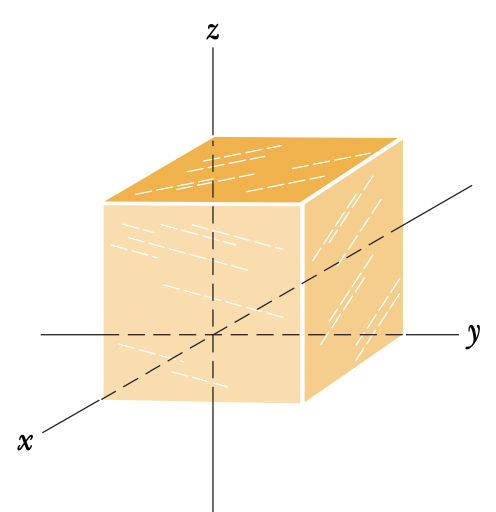
\includegraphics[scale=0.6]{qfig3-1.png}
  \caption{\textbf{문제 2}}
  \label{fig:1}
\end{figure}
\begin{itemize}
\item[(가)] $6.00\,\hat{\bm{i}}$,
\item[(나)] $-2.00\,\hat{\bm{j}}$,
\item[(다)] $-3.00\,\hat{\bm{i}}+4.00\,\hat{\bm{j}}$  
  라면 오른쪽 면을 통과하는 전기장 다발은 각각 얼마인가?
\item[(라)] 정육면체를 통과하는 알짜 전기장 다발(net electric flux)을
  구하여라.   
\end{itemize}
\vspace{0.5cm}

\noindent{\bf 풀이 : }
\begin{itemize}
  \item[(가)]
  \item[(나)]
  \item[(다)]
  \item[(라)] 
\end{itemize}
\vspace{0.5cm}
\noindent {\bf 문제 3 [20pt].} 그림~\ref{fig:2}처럼 질량이 1 mg이고
전하가 $q=2.0\times 10^{-8}$ C로 균일하게 분포되어 있는 작은 부도체
공이 얆고 전하가 균일하게 대전된 부도체 면과 $\theta=30^\circ$의
각을 이루며 부도체 실에 매달려 있다.  
\begin{figure}[htp]
  \centering
  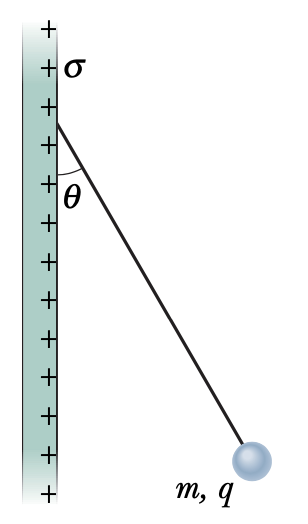
\includegraphics[scale=0.6]{qfig3-2.png}
  \caption{\textbf{문제 3}}
  \label{fig:2}
\end{figure}
이 절연체 판이 무한히 크다고 가정하자. 이와 같은 평형을 만들 수 있는
면전하밀도 $\sigma$를 구하여라.
\vspace{0.5cm}

\noindent{\bf 풀이 : }

\vspace{0.5cm}

\noindent {\bf 문제 4 [50pt].} 그림~\ref{fig:3}에서 상자 모양의 가우스
면이 $+24.0\varepsilon_0$ C의 알짜전하를 포함하고 전기장
$\vec{E}=[(10.0 + 2.00x)\,\hat{\bm{i}}-3.00\,\hat{\bm{j}}+
  bz\,\hat{\bm{k}}]$ N/C 안에 놓여 있다. 
\begin{figure}[htp]
  \centering
  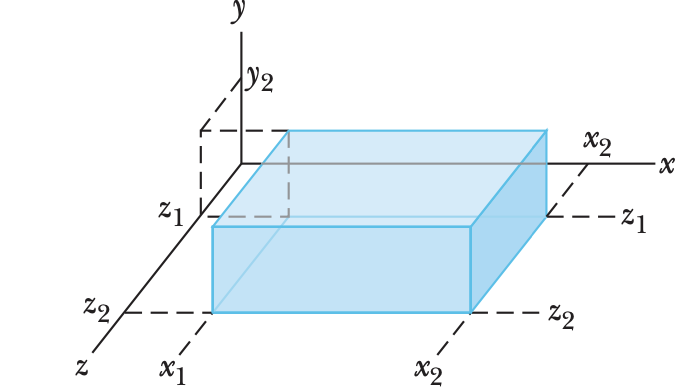
\includegraphics[scale=0.6]{qfig3-3.png}
  \caption{\textbf{문제 4}}
  \label{fig:3}
\end{figure}
$x$, $z$은 미터 단위로
  주어지고, $b$는 상수이다. 밑면은 $xz$평면이고, 윗면은 $y_2=1.00$ m를
  지나는 수평면이다. $x_1=1.00$ m, $x_2=4.00$ m, $z_1= 1.00$ m,
  $z_2=3.00$ m일 때, 상수 $b$는 얼마인가? 
\vspace{0.5cm}

\noindent{\bf 풀이 : }

\vspace{0.5cm}

\end{document}